\chapter{Algorithms implementation}
\label{chapter:implementation}

The actual implementation of the designed algorithms introduced in Chapter~\ref{chapter:methods} is now extensively described. 
As anticipated in the previous chapter, here all the details of the developed phases of the project are deeply analysed and explained. 
A path similar to the one followed during the actual designing of the algorithms is used for outlining the whole project.\\
First of all, the preparatory tests performed for evaluating the feasibility of the conceived idea are reported and explained. 
Subsequently, the focus moves on the two main methods designed, the derivative based one and the strategy based on the standard SGM pipeline.
After that, the side phases of the work are presented. 
The pre and post-processing operations are accurately defined and the comparison among the different filtering operations are carried out.

\section{Preparatory and testing phase on MATLAB}
\label{section:prep-pahse-matlab}

\begin{figure}[t]
	\centering
	\subfigure[Left ground truth stereo test image overlapped by a simulated point grid]{
 		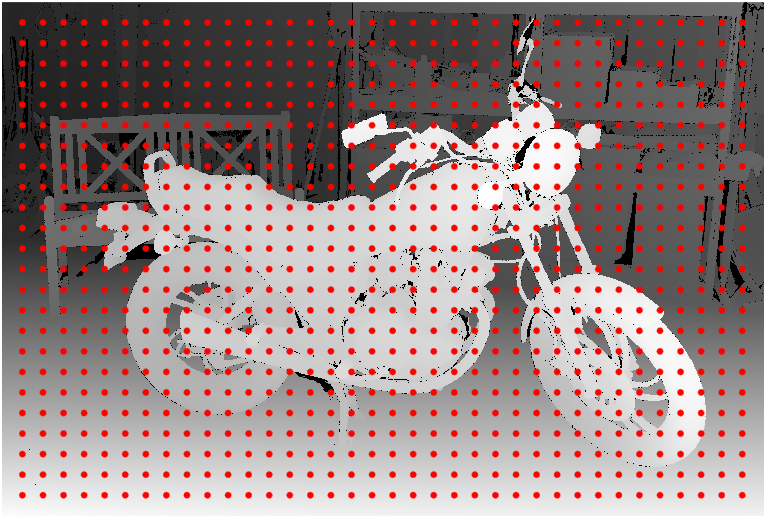
\includegraphics[width=0.4\textwidth, height= 5cm, keepaspectratio]{images/disparity-plus-grid-test-left-01.png}
 		\label{fig:test-matlab-left-01}
}
	\subfigure[Right ground truth stereo test image overlapped by a simulated point grid]{
 		 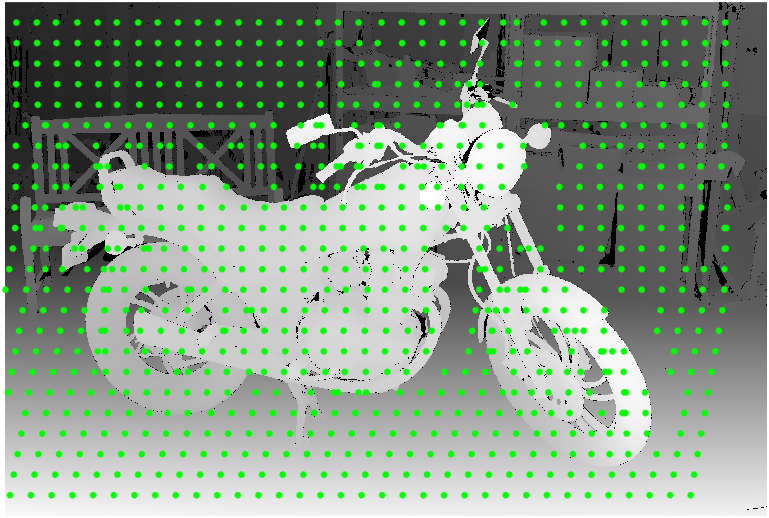
\includegraphics[width=0.4\textwidth, height= 5cm, keepaspectratio]{images/disparity-plus-grid-test-right-01.png}
 		 \label{fig:test-matlab-right-01}
}
\caption{Ground truth images from the Middlebury dataset used for the initial testing phase}
\label{fig:test-matlab-01}
\end{figure}

As anticipated in Chapter~\ref{chapter:methods}, the first phase of the project can be mainly considered as a researching stage.
As a matter of fact, exploiting the stereo images from the Middlebury 2014 dataset, some tests have been performed to obtain an estimation of the feasibility of the conceived idea.\\
Therefore, as Figure~\ref{fig:test-matlab-01} displays, ground truth images have been initially used.
Thus, a point grid, similar to the one generated with the LadiMo device, has been simulated and overlapped to the input images.
In particular, as the difference between Figure~\ref{fig:test-matlab-left-01} and Figure~\ref{fig:test-matlab-right-01} illustrates, to have a reliable simulation of the 3D point cloud generated by the device, the only grid that was actually defined was the one over the principal image, i.e. the left one.
As a matter of fact, as defined in section~\ref{section:stereo-device}, the hardware exploited in the project is provided with only one laser projector.
Therefore, this allows to utilize the produced point cloud only over one image\footnote{Technically speaking the initial cloud of point created through the device can be independently related to both of the image, depending on which is used as the reference one, just applying the correct transformation between the laser and the principal image coordinates systems}.
After that, those input data, together with the grayscale stereo pair, have been employed in a stereo matching pipeline to recover a disparity map of the analysed scene.\\
In order to acquire useful baseline data regarding the practicability of the thought strategy, tests and analysis over the different areas of the main loop of the algorithm have been investigated.
Actually, this research has been performed with a precise method. \\
First of all the stages of a standard stereo matching method, as defined by Scharstein and Szeliski in~\cite{Scharstein2001}, have been separately examined. 
Thus, in order to do this in a reasonable way, the literature regarding both standard and novel stereo matching algorithm has been studied and the main features of the designed algorithm checked out. 
As an example, if the matching cost phase is taken into account, different approaches are presented in the literature for evaluating the similarity among the image pixel values for the respective disparity levels. 
As a matter of fact, as introduced in Chapter~\ref{chapter:methods}, the Hamming distance between corresponding pixels can be exploited to determine that measure. 
In relation to that, different algorithms exist to apply a transformation to the input images, making them available for an appropriate implementation of the aforementioned matching cost calculation.
For the actual tests carried out, local methods have been mainly analysed, being more appropriate for the type of data available and for the purposes of the designed strategy.\\
Therefore, as matching cost measures, simple operations have been initially taken into account, such as the sum of absolute differences (SAD) and the sum of squared differences (SSD). 
Moreover, more accurate methods have been later evaluated, i.e. the Rank transform, and its improved version, the Complete Rank transform, broadly discussed in~\cite{Demetz2013}.
Then, the Census transform and the Center-Symmetric Census transform proposed by Spangenberg et al. in~\cite{Spangenberg2013} have been investigated.
Considering all of those algorithm, it resulted that the most suitable methods are equivalently the Rank and the Census transform.
In fact, being these non-parametric transformations, they are not sensitive to changing in lightning inside the environment, thing that usually happen when managing real industrial areas. 
Considering that, at the end the Center-Symmetric Census transform has been chosen because of its reliability, which is comparable to the aforementioned methods, and for the fact that it uses a lower amount of bits to describe the single pixel value compared to the standard Census transform.\\
During this phase of testing, the decision was to run a single pipeline of an \textit{SGM-based} algorithm, whose aggregation cost phase would be based on the four orthogonal directions. 
Moreover, another operative choice was to use the whole image for the complete execution of the designed method.
Therefore, it was thought that, at least for this researching phase, it would be meaningless to define a hierarchical implementation of the code, where the image is initially downscaled and subsequently scaled up again in order to make the execution faster, as made by Hermann and Klette in their application of the SGM algorithm~\cite{Hermann2013}.\\
At the end of this \textit{research} section of the project, the results did not show an exact path to follow, meaning that there was not a clear improvement over the normal SGM-based approach by using the initial set of grid point, compared to the MATLAB built-in method used as baseline. 
Specifically, the disparity image obtained was actually lower in accuracy compared to the method implemented in MATLAB by Eric Psota and available at the website of the Middlebury stereo dataset \footnote{\href{http://vision.middlebury.edu/stereo/submit3}{links Middlebury College Stereo}} and to the MATLAB built-in method \texttt{disparitySGM()}. 
Moreover, the developed implementation was quite slow, if correlated to the benchmark of most of the standard SGM-based methods. \\
However, some considerations should be proposed regarding that outcome. 
First of all, the algorithm designed runs iteratively, that is no parallel loop is coded to make the execution faster.  
This is, in fact, explained by the decision of being interested in the relative performance among the own designed methods. 
Furthermore, any sort of GPU enforcing was not used. 
Hence, it was quite expected to not obtain good performance.
Therefore, the thought strategy was evaluated as feasible and, additionally, the exploiting of proper initial data provided by the stereo camera would likely be an enhancement to the overall performance of the algorithm. 
Moreover, the derivative based algorithm has not been initially tested, however, considering its main idea, it should theoretically give accurate results in a reasonable computational time.

\section{Derivative based method implementation}
\label{section:derivative-based}

Verified the feasibility of the considered strategy, the project design shifted to the actual algorithm development. 
Therefore, exploiting the OpenCV libraries and using the images from the Middlebury 2014 dataset, the derivative based method started to be implemented in a C++ code. \\
In the initial phase of its designing, the simulated grid based on the ground truth images was still used to obtain the input point cloud data.
As a matter of fact, the only practical advantage of employing such simulated data stands on the amount of noise that they contain.
As a matter of fact, an appropriate comment to that strategy would be that, once the real data from the device would be used, the result would probably be worse in terms of overall accuracy. 
Anyway, at that initial stage of the algorithm development, the interest was focused on comparing the performance of the pure SGM-based and the derivative-based implementations. 

\subsection{General features of the method and simulated grid specifications}
\label{subsection:general-feature-der-method}

\begin{figure}[t]
	\begin{center}
		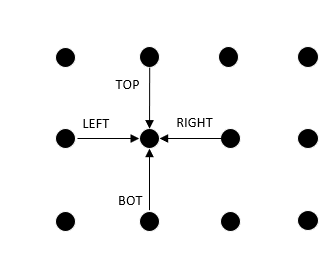
\includegraphics[width=.8\textwidth, height=5cm, keepaspectratio]{images/grid-subwindow-detail}
\caption{Detail of a point grid patch where a set of neighbouring points is highlighted}
\label{fig:grid-subpatch}
	\end{center}
\end{figure}

\begin{figure}[t]
	\begin{center}
		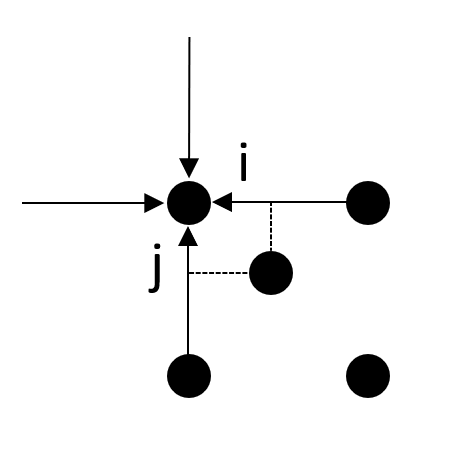
\includegraphics[width=.8\textwidth, height=5cm, keepaspectratio]{images/point-estimation-detail}
\caption{Detail of a point grid patch where the estimation of a new point at relative coordinates $i$ and $j$ is performed}
\label{fig:subpatch-estimation}
	\end{center}
\end{figure}

The so called derivative-based method, which arises to be both efficient and generally accurate, based its strength on the sparse point cloud gained through the structured light assisted stereo camera.\\
The main features of that algorithm are now precisely described.
Moreover, attention is focused on the conventions utilized to define the main parts of the method and on the functions created for obtaining the 3D point estimations over the initial laser grid. 
Subsequently, some fundamental sections of the designed implementation are more broadly described, thus to provide to the reader a complete understanding of the work done. \\
For this reason, the analysis starts by considering a simulated grid of points, which was defined in the C++ code in order to initially mimic the real laser grid generated by the LaDiMo device. 
In fact, the actual grid of points generated by the company device is not perfectly parallel to a vertical plane, as the simulated one, contrarily it is tilted at $16.7^{\circ}$ w.r.t. the vertical axis.
However the approach followed, as aforementioned, does not invalidate the outcome obtained through all the designing process of the method.
Instead, it is a reasonable strategy for achieving some initial temporary results, which can then provide a guidance to the following phases of the whole process.\\
Therefore, let us consider the entire point cloud as a regular grid where each point is defined by its coordinate in space.
Additionally, it can be also thought that the corresponding 2D coordinates in the reference image plane can be easily retrieved using the camera projection matrices.
Hence, if a neighboring set of four points is taken into account, as highlighted by Figure~\ref{fig:grid-subpatch}, the local derivative vectors for all the considered coordinates can be easily calculated.
This estimation of the derivative is extremely useful for the following reasons.
First of all, they are, actually, exploited to generate the estimations inside each grid sub-region.
Moreover, they can be employed to evaluate if, inside the specific patch of points, there could be an edge of some shape. 
In this latter case, the magnitude of the $Z$ component of the derivative vector will, in fact, be higher than a set threshold, which can be defined looking at the average values of the $Z$ coordinate of the grid points.\\
Therefore, explaining the project design procedure implemented, it can be summarized as follows.
Initially, for each one of the points in the grid the internal and external derivatives have been calculated with respect to its four neighbors, as the arrows in Figure~\ref{fig:grid-subpatch} underline. 
This means that each point will have, then, four distinct set of local derivatives, for both the internal and the external ones, conventionally defined as follows:
\begin{itemize}
	\item \textbf{from top:} derivative between the specific point and its top neighbor;
	\item \textbf{from boottom:} derivative between the specific point and its bottom neighbor;
	\item \textbf{from left:} derivative between the specific point and its left neighbor;
	\item \textbf{from right:} derivative between the specific point and its right neighbor.
\end{itemize}
In these definition a neighbor to a point is defined with the subsequent rule. 
Let us consider a point, which is classified through the grid coordinates $r$, along the row grid direction, and  $c$, along the column direction. 
Its neighboring points are, hence, identified by:
\begin{itemize}
	\item \textbf{top} neighbor: with coordinates $r - 1$ and $c$;
	\item \textbf{bottom} neighbor: with coordinates $r + 1$ and $c$;
	\item \textbf{left} neighbor: with coordinates $r$ and $c - 1$;
	\item \textbf{right} neighbor: with coordinates $r$ and $c + 1$;
\end{itemize}
Using that scheme the four derivatives estimated for each point will contain the difference between the actual point  \textbf{\textit{full location components}} and the ones of the relative neighbor regarding.
In the implemented code, the introduced \textbf{\textit{full location components}} are in the order: the $X$, $Y$ and $Z$ space coordinates of the point, in meters, the $x$ and $y$ components of the point projected in the principal image plane, therefore they are measured in pixels, and finally, $d$ is the disparity value, in pixel, related to the depth of the point, which can be evaluated through equation~\ref{eqn:disparity-depth} and adding the relative \textit{disparity offset} if required.
This gain was, in fact, necessary when using the data from the Middlebury dataset, where the relation between the ground truth disparity values and the corresponding depths is defined as in the equality~\ref{eqn:middlebury-depth-disp}
\begin{equation}
	\label{eqn:middlebury-depth-disp}
	Z = \frac{B \cdot f}{d + d_{offs}}
\end{equation}
where, as in~\ref{eqn:disparity-depth}, $B$ is the camera baseline, $f$ the respective focal length and $d_{offs}$ the disparity offset, which is the different between the $x$ coordinate of the principal points, as following clarified:
\begin{equation}
	\label{eqn:doffs-equality}
	d_{offs} = c1_x - c0_x
\end{equation}
where $c1_x$ is the $x$ coordinate of the principal point for the support camera, while $c0_x$ is the $x$ coordinate of the principal point for the main camera.\\
Therefore, let us now consider to estimate an unknown point inside a subregion of the whole grid, that was decided to be identified by 4 points, as Figure~\ref{fig:subpatch-estimation} displays.
The final 3D coordinates of the new point will be, at first, defined by four different estimations, each one related to the four corners of the grid subwindow, as follows.

\begin{subequations}
\label{eqn:point-patch-estimation}
	\begin{align}
		est_{TL} = TL + i \cdot der_{from-left} + j \cdot der_{from-top} \\
		est_{TR} = TR + (i-1) \cdot der_{from-right} + j \cdot der_{from-top} \\
		est_{BL} = BL + i \cdot der_{from-left} + (j-1) \cdot der_{from-bottom} \\
		est_{BR} = BR + (i-1) \cdot der_{from-right} + (j-1) \cdot der_{from-bottom}
	\end{align}
\end{subequations}

where $TL$, $TR$, $BL$ and $BR$ respectively point to the estimation done with respect to the top-left corner of the grid sub-window, the top-right corner, bottom-left and bottom-right corner. 
Then, $i$ and $j$ are the relative $x$ and $y$ coordinates of the estimated point, whose values range between 0 and 1.
Finally, in the notation employed, $der_{dir}$ stands for the different derivative vectors related to each corner point and visualized by the arrows in Figure~\ref{fig:subpatch-estimation}.
Here, in order to keep the generality of the notation, no distinction has been made between internal and external derivatives.
As a matter of fact, in both cases the calculation performed are actually the same.
The difference only interests the specific values of the vectors and the analysed case, considering that the internal derivatives are in general used.
The external ones are exploited when some sort of edge is detected inside the analysed patch, after having verified that other edges are not located on the close neighborhood of the targeted subwindow. \\
Once, these estimations are achieved exploiting the derivatives, as equations in~\ref{eqn:point-patch-estimation} define, the best evaluation is obtained by calculating each matching cost between the corresponding pixels between the stereo images. 
The matching cost is determined following the subsequent routine.\\
In relation do this, it should be reported that, due to the researching aspect of this project, lots of changing have been made to the code.
Therefore, to provide a clear explanation of the decisions made and the procedure followed, which, otherwise, could appear somehow winding, all the relevant changes to the functions used are disclosed. 
Beside this brief comment about the designed code, the best, among four, estimation of the new grid point is such evaluated.\\
The estimation provides the values of the 3D coordinates of the calculated point and its disparity.
The point location is, then, projected through the camera matrix to the reference image (usually the left image) pixel coordinates and the corresponding position in the support image is determined using the estimated disparity value. 
At this point the matching cost is computed as the absolute difference between the intensity values of the analysed pixels in the left and in the right image planes. 
However, this kind of measure appears to give weak results. 
As a matter of fact, the main problem was that, in some situations, the estimation labelled as the best one actually contained a value of disparity doubtful, if compared to the one of the point's closest neighbors.  
Moreover, this generally happened in texture-less regions, where it is obviously more difficult to make accurate estimations.\\
To overcome this problem, a penalty value was added to each partial estimation. 
Specifically, that value was weighted linearly basing on the distance between the estimated point and the corresponding corner. 
In this manner, the estimation, related to the disparity and to the coordinate values of the closest corner, is most likely to be addressed as the best one.
Once the best estimation for each new point is calculated, the evaluated values of the 3D point coordinate are processed, applying a morphological filter, in order to remove undesired noise and smooth out the overall data. \\
The estimation procedure just described is not actually able to handle all kind of situations, concerning the provided input objects.
In fact, incorrect values used to be estimated in subregions affected by edge features, and thus occlusions. \\
Therefore, to correctly manage these situations, multiple cases have been defined, regarding the edge cases. 

\subsection{Edge cases and penalty values discussion}
\label{subsection:edge-cases-and-penalties}

At first, four main conditions have been distinguished. 
These comprise the possibility to do not have any type of edge inside a grid subregions, the existence of a vertical edge in the patch, an horizontal edge case and finally a so called \textit{undefined} case has been defined.\\
Therefore, in each one of these situations, the point estimation procedure differs slightly, so that the aforementioned linear penalty can be more wisely set.
Regarding this two distinct values of the penalty have been employed, a lower and a higher value.
In fact, because it is not efficiently possible to correctly estimate the position of the potential edge, the choice of the correct estimation has to be somehow driven by exploiting the linear penalties. \\
Moreover, to identify the correct type of edge, the derivatives have been exploited and, specifically, the magnitude of the $Z$ component of the vector. 
Basically, a general edge case, which is equivalent to the \textit{undefined} condition, is initially verified by computing the absolute difference between the $Z$ components of all the possible couples of corners, i.e. the $Z$ value of the local derivatives, and comparing that with a pre-determined threshold, which is related to the average depth value of the initial points of the grid. \\
Therefore, during the algorithm pipeline, the possibility of having an edge feature inside the specific patch is initially checked.
Then, if the depth values of the four corner are almost equivalent, this means that the area is actually planar.
Thus, in this situation, a fast interpolation method is run, so that the overall computation can be even faster.\\
On the contrary, if a vertical or an horizontal edge is found, the small and big penalties are used accordingly.
For example, if the edge is vertical, the small penalty will be multiplied to the relative $y$ coordinate of the estimated point, instead the big penalty will weight the $x$ coordinate.\\
Finally, for the undefined case, the penalty weight is equivalent in both directions, $x$ and $y$, and its magnitude ranges between the two previously defined values. \\
Those three different edge cases are the one initially tested. 
However, later appeared that a more meaningful strategy should be based on the definition of two grater categories, which would comprise the cases described above.
These two bigger classes describe, thus, \textbf{\textit{soft}} and \textbf{\textit{strong}} edges. 
In fact, results of tests done with dataset images show that employing a single threshold for the depth difference and focusing only over the edge direction was not entirely adequate. 
As a matter of fact, in a generic scene different types of objects exists. 
Therefore, adapting the edge analysis to the object distances, for example between the whole foreground and the background and between multiple objects of the foreground, that would give a smoother and more accurate final dense 3D point cloud.

\subsection{Derivative computation and sanity check}
\label{subsection:derivative-computation}

The core of the estimations are, actually, the local derivatives computed for each point of the grid. 
Basically, each grid point contains four vectors, which are the local derivatives between the reference point and its four orthogonal neighbors. \\
Initially the mere derivatives have been calculated as pointing towards the reference point, like Figure~\ref{fig:grid-subpatch} shows. \\
However, it came out that this procedure was not enough accurate, to generate a proper dense 3D point cloud.
Therefore, a \textit{sanity check} has been later defined inside the derivative calculation pipeline to achieve preciser computation of the local derivatives, especially for the grid sub-patches where edges are most likely to be found.\\
Moreover, a higher accuracy of the final result has been achieved when evaluating, for each grid point, two slightly different types of derivative vectors.
Specifically, \textbf{\textit{internal}} and \textbf{\textit{external}} derivatives. 
This distinction allowed to achieve faster and more accurate results, especially when dealing with edges in the grid subregion. 
Precisely, if the presence of an edge is verified for the considered patch, the external (with respect to the sub-window) derivatives were used.
Otherwise, exploiting the internal derivatives the computation could be made faster, being them equal in couple among the corners of the patch. \\
Referring to what introduced at the end of Section~\ref{subsection:edge-cases-and-penalties}, in the latest implementation designed, the estimation process is mainly driven by the edges analysis. 
As aforementioned, the test results demonstrate that a distinction based only upon the edge shape is not enough to reach a good degree of accuracy.
Therefore, the analysis cases have later been defined basing on the strength of the edges between the objects in the scene.\\
Hence two different thresholds have been so determined. 
The first is used to identify occlusions that basically occur between foreground objects and the background. 
These have been designated as \textbf{\textit{strong}} edges. 
Differently, the other case is specified as the \textbf{\textit{soft}} edges case.
This is related to occlusions happen between parts of the same object at different values of depth, as could be between the chin and the neck of a person.\\
Moreover, on top of this first level of edge selection, the following cases have been then defined, which are correlated to the specific value of the penalty.
Precisely, they are \textit{pure vertical} and \textit{pure horizontal} edges, for which it should happen that the depth values of the corners are equals in couple.
Then, there are some particular cases, which have the scope of leading the disparity estimation to a higher level of accuracy.
They are: \textit{diagonal top left}, \textit{diagonal top right}, \textit{diagonal bottom left}, \textit{diagonal bottom right}.
Furthermore, there is the undefined case, which is triggered when the potential edge found in the subregion has a strange shape.\\
Taking now into account the actual estimation functions, these are slightly different for the aforementioned edge cases identified.
Summing up the overall procedure, it can be said that, the main distinction, which guides the whole process is the first one, that is the one that distinguish among, strong, soft and no edges.
Then, for all the subcases, the main difference stands on the values and order of the penalties. \\
Hence, in the \textit{no edges} case, four temporary estimations are performed for each new grid point by carrying out a linear interpolation, which exploit the \textit{internal} derivative vectors.
Then, for the other two main cases, the procedure is generally the same. 
In fact, the fundamental scope of distinguish between those types of occlusions is to make the final outcome smoother. \\
Thus, when dealing with edges, at first the algorithm checks for each temporary estimation, that is for each subregion corner, if there could also be edges in the neighborhood outside of the region. 
If this is false, a linear interpolation is computed employing the \textit{external} derivatives.
Otherwise, the interpolation is done with the \textit{internal} derivatives and only for the $x$ and $y$ pixel positions. 
Instead, the depth value is matched with the one of the corresponding corner, thus to enhance the smoothness of the final result.
Regarding the $X$, $Y$ and $Z$ values, these can be easily recovered from the previously estimated pixel coordinates and disparity, by exploiting the camera projection matrices and the relative equations. 

\section{Semi-Global Matching based method implementation}
\label{section:sgm-based}

The other implemented method based on the initial grid of points follows more closely the standard stereo-matching structure.
Moreover, it does not distinguish between \textbf{\textit{strong}} and \textbf{\textit{soft}} edges, but the different cases are identified only considering the shape of the potential edge present inside the subwindow. \\
Therefore, this algorithm initially computes the \textit{matching cube cost} for the specific grid patch. 
The difference between the standard SGM method stands on that cube, whose third direction does not generally contains continuous values of the disparity.
On the contrary, those values are defined by the sub-window corners, whose disparity define the levels of the cost cube.\\
Therefore, if no edge is found, only the matching cost part of the stereo algorithm is carried out.
Otherwise, the aggregation cost phase is implemented.
In this latter case, the cost is actually aggregated only on the direction orthogonal to the shape of identified edge, thus to make the implementation faster.
As a matter of fact, let us consider a specific sub-patch in the principal image and the pixels that belong to it.
Let us, then, assume to identify a vertical edge inside that subregion.
It would be worth nothing to aggregate the matching costs related to each pixel along the vertical direction.
The differences among the intensity values of the pixel along that direction would, in fact, be extremely lower than the variations along the orthogonal direction.
Therefore, because in general the matching costs are aggregated along all of the four orthogonal directions, the values along the path orthogonal to the edge will weight more.
While the costs along the path parallel to the edge will have less relevance, technically speaking.
Therefore, it would be worth nothing to aggregate the cost along all the four directions, obtaining as the only outcome an increasing in the algorithm complexity.
On the contrary, if a particular edge is determined inside an image patch, it would be more efficient to run the aggregation cost step along the two orthogonal directions only.\\
At the end of the pipeline simple post-processing operations are performed over the obtained data, as done for the other algorithm.
Considering the overall method, it result to be give a denser point cloud compared to the previous method. 
However, its computational time is extremely higher.
This is clearly due to the fact that this algorithm estimates each single pixel inside the specific subregions.
Contrarily, in the \textit{lightweight} strategy the number of samples that the user wants to estimate can be adjusted. 
In this way the trade-off between accuracy and resources utilization can be externally defined. 

\section{OpenCV built-in Semi-Global Block Matching algorithm}
\label{section:opencv-sgm-method}

In comparison to the designed algorithms, it was decided to generate some results exploiting the Semi-Global Block Matching method available in the OpenCV library.
This was mainly done to set a baseline outcome, extremely useful for comparing the disparity images obtained.
As a matter of fact, the performance and the accuracy of the OpenCV built-in algorithm were essentially related to the outcomes carried out applying the simulated grid procedure.\\
Therefore, a clear measure in terms of both computational time and absolute accuracy has been available during project development, thus to have a transparent benchmark over the potential of the designed strategy.

\section{Pre-processing testing and analysis}
\label{section:pre-processing-impl}

The pre-processing phase can be ideally divided in multiple parts.
First of all, general operations have been applied for both estimation methods in order to remove noisy components from the stereo pair and from the ground truth images, when exploiting the simulated grid for the estimations.
Then, a section of the pre-processing phase can be considered the importing of all the necessary calibration data and the creation of a sort of look-up table, which was used together with the grid of points.\\
On the contrary, when working with the real data coming from the LaDiMo stereo device, some initial operations have been necessary to clean up \textit{bad} point values and for estimating some of the missing data, which would be determined without losing in accuracy. \\
Regarding the image pre-processing, different noise removal filters have been tested over database images, in order to understand which would provide the best trade-off in most of the cases. 
Median and bilateral filters appear to be, almost equivalently, the best choice for smoothing away the noise while loosing the smallest amount of information from the input images, because of the peculiarity of being edge preserving filters. \\
Considering the others pre-processing operations implemented in the algorithm, they depend on the condition of working or not with the simulated grid.

\subsection{Look-up table and point grid pre-processing}
\label{subsection:grid-preprocessing}

Therefore, for the initial testing phase of the algorithm designing, when multiple tests have been carried out using the images from the Middlebury dataset, a look-up table has been defined in order to ensure a fast data retrieving. 
This structure has been easily built by progressively numbering the simulated gridpoints, so that their values correspond to the row index of the \textit{complete data matrix}.
That is the matrix that actually contains the space and relative pixel information for all the point belonging to the initial grid, i.e. $X$, $Y$ and $Z$ in meters or millimetres and $x$, $y$ and \textit{disparity} in pixels. \\
Regarding the implementation run over the real data, instead, some pre-processing operations have been necessary to adjust the initial device data, which were not always perfect. 
As a matter of fact, a low percentage of points of the laser grid, which ranges between 2.7 and 3.2 \% depending on the specific scene (\textbf{check the error percentage, not sure}), was missing. 
It used to happen that the points were, in fact, not visible in the grid, as overlapped to the raw image, however, the raw data coming from the device present their grid coordinates alone, without any further information about their location.
Therefore, those points were labelled and ordered by the algorithm running on the device, however no data were available regarding their space or image positions.
This behaviour usually happened for the points located close to edges, and thus close or even above occlusions. 
In those cases the accuracy of the device drops locally and the provided results are, in fact, missing. 
So that, pre-processing procedures were necessary in order to reduce the percentage of initial errors, which usually diminishes between 0.8 and 1.2 \%, depending on the density of missing data in the occluded regions.
However, even if in general the error dropping was not high, it marginally impacts on the overall performance of the algorithm, providing more accurate results in regions interested by edges and, hence, occlusions. \\
Specifically, two main operations have been performed over the initial raw data to reduce the errors.
First of all, the grid points have been entirely analysed in order to identify the area where the percentage of missing data were low enough to allow a highly accurate reconstruction of the values of those point.
As a matter of fact, a non perfectly exact estimation would carry errors over all the algorithm pipeline, which is a not desirable outcome. \\
Hence, where enough raw data were present in the neighborhood of occlusions, the estimations have been performed by evaluating a fast yet accurate linear interpolation exploiting the four closest neighbors to the specific point. 
Related to this, it was proved that performing a bilinear interpolation or using a weighted average to estimate missing values had the same grade of efficiency as the simple average, employing at least two orthogonal neighbours. \\
After the data filling a minor percentage of missing values was generally still present. 
Therefore, before running the algorithm those grid points was removed, being useless in the whole pipeline.
In regard to this, it is worth to make notice that the \textit{bad} points were in most of the cases almost the 2.5 - 3 \% of the entire grid data. 
Therefore, it can be concluded that the value would not affect sensibly the overall accuracy of the final result and that a high density of point could be certainly reached with the available amount of raw data.\\
On the other hand, the application of a high expensive method, which would probably only provide an additional error reduction of the 0.5 \% would be worth noting and it would most likely affect the speed of the algorithm, without providing a reasonable improvement of the density of the final point cloud.
Therefore, it was considered beneficial to apply the aforementioned data recovering, over the condition of filling the missing data with a high accuracy. 
Considering, in fact, that the initial amount of errors was generally acceptable for achieving final accurate results, a mild data retrieving, which would not affect the performance of the algorithm while slightly increasing the amount of initial information, has been evaluated as valuable for the whole method.

\subsection{Image undistortion and rectification}
\label{subsection:img-undist-and-rectific}

\begin{figure}[t]
	\centering
	\subfigure[Left distorted raw image]{
 		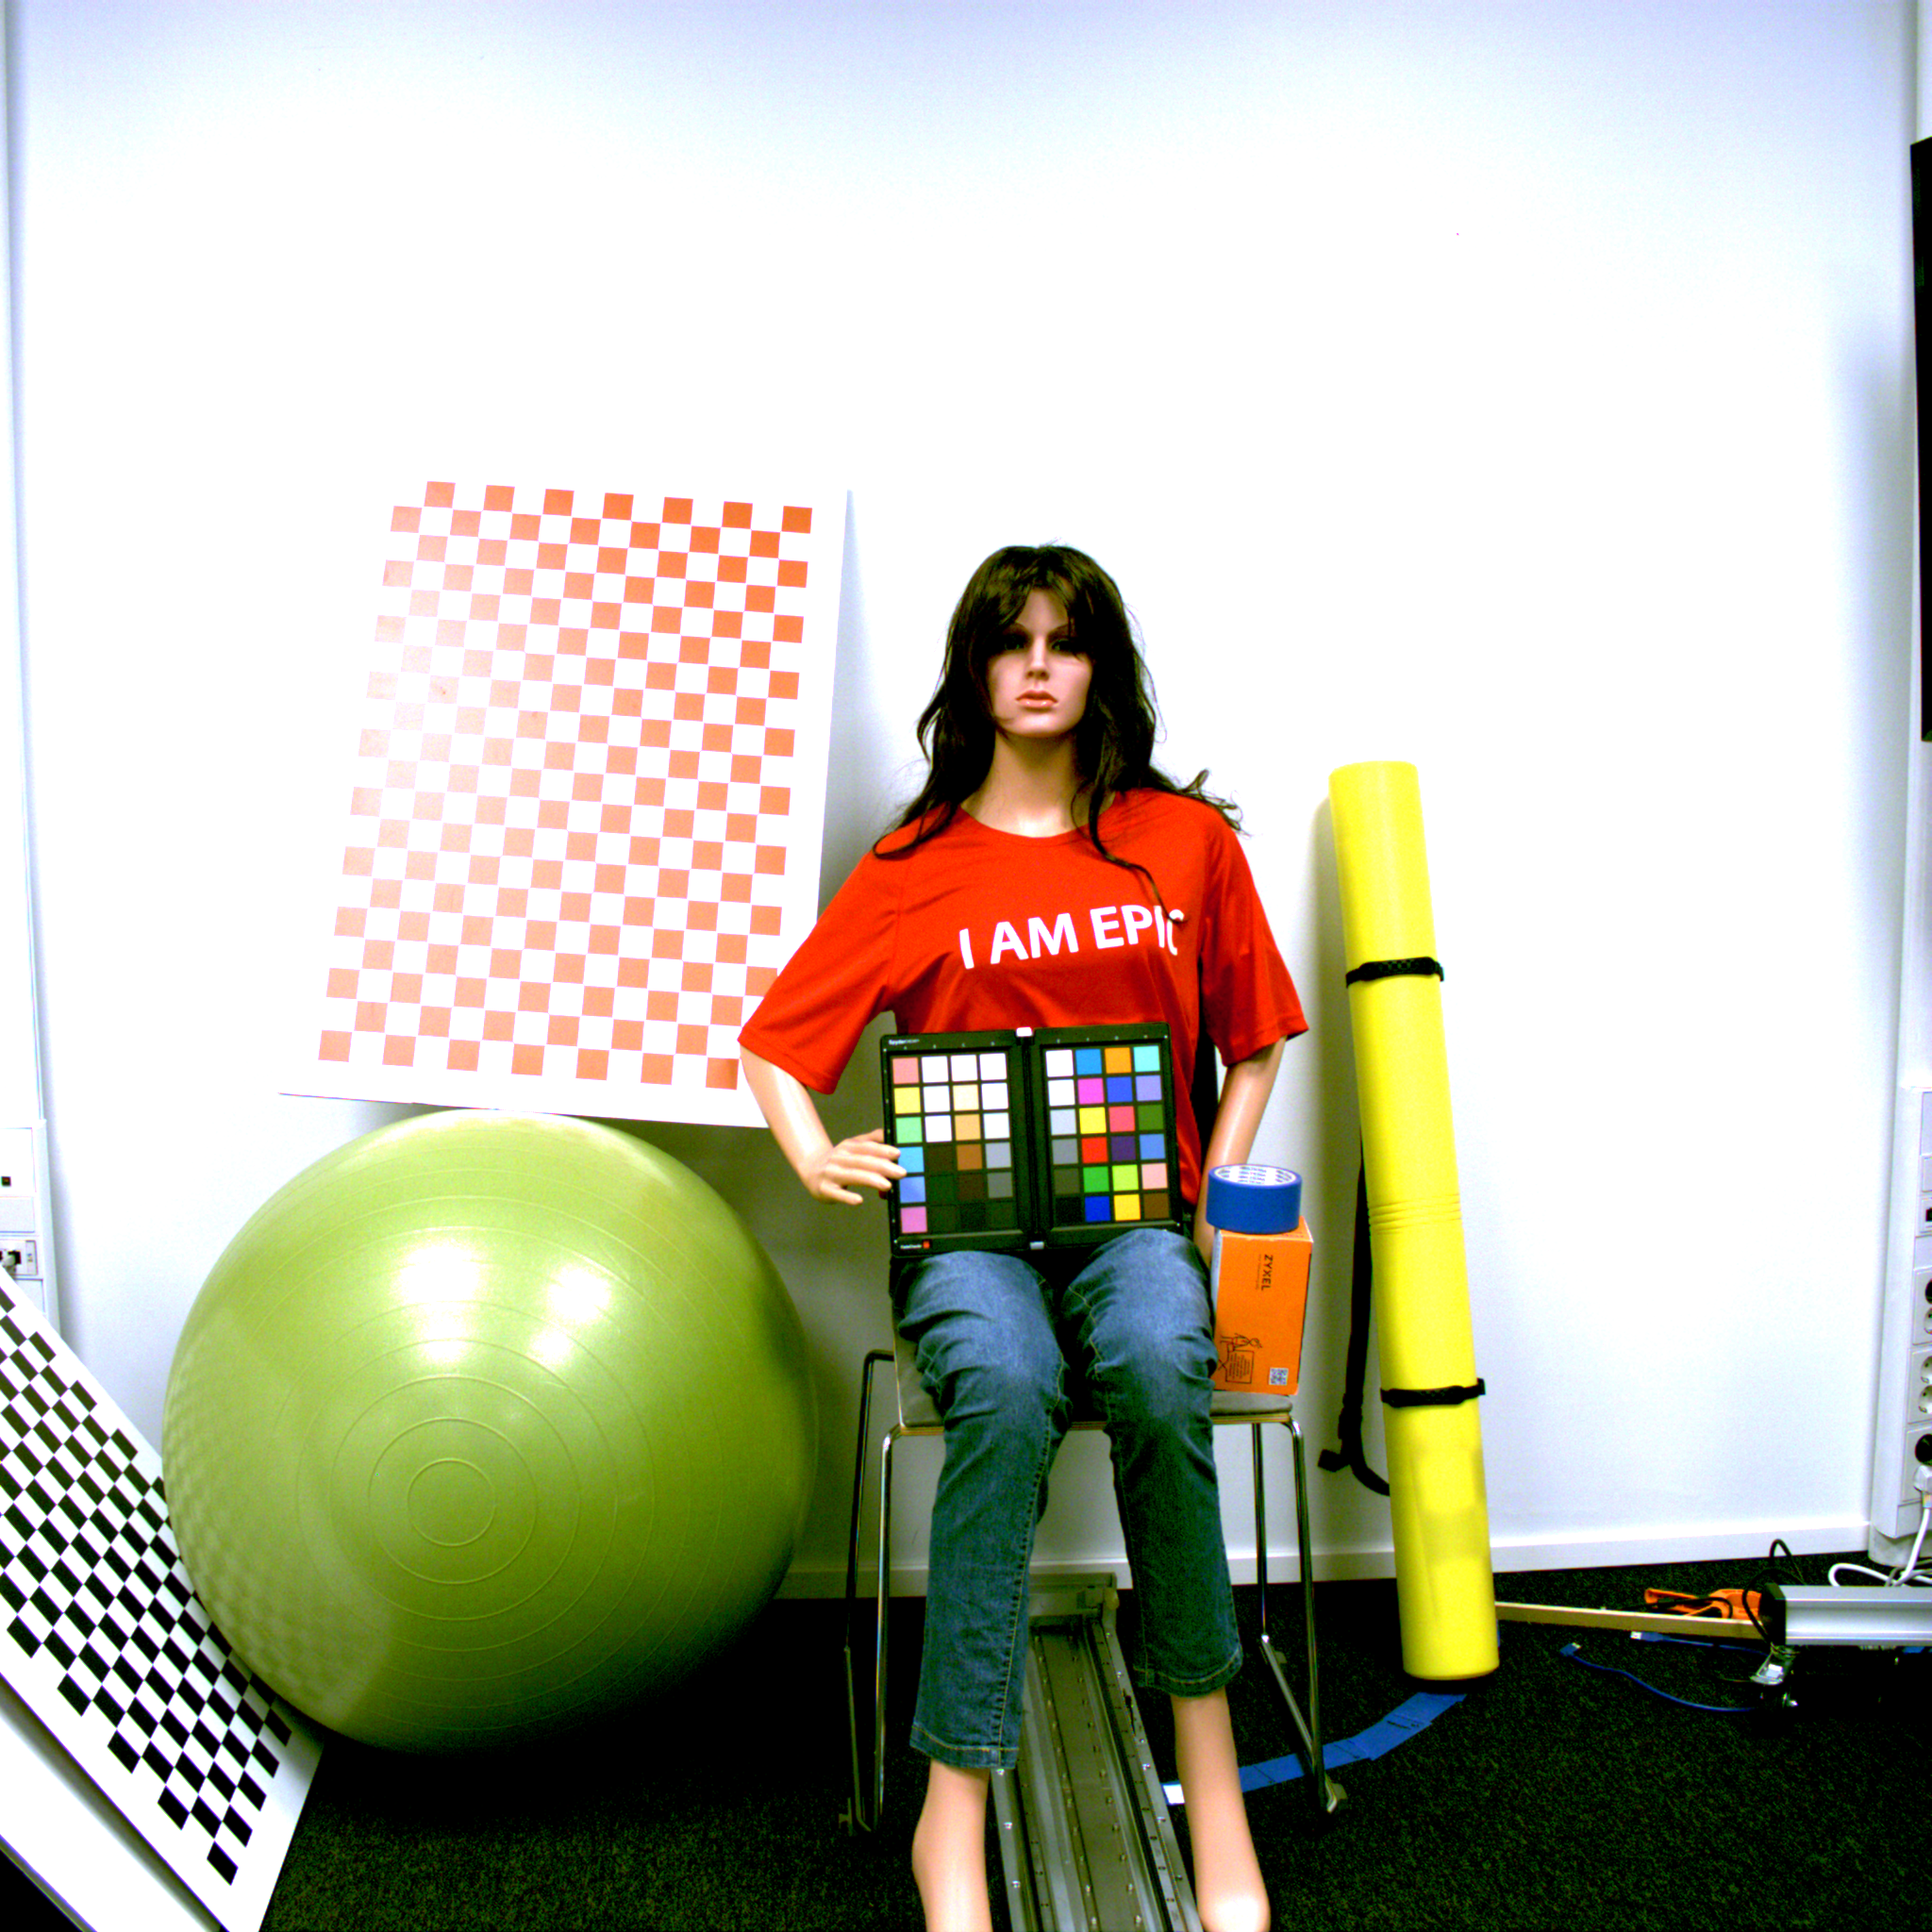
\includegraphics[width=0.4\textwidth, height= 5cm, keepaspectratio]{images/input-image-raw-left.png}
 		\label{fig:distort-raw-left}
}
	\subfigure[Right distorted raw image]{
 		 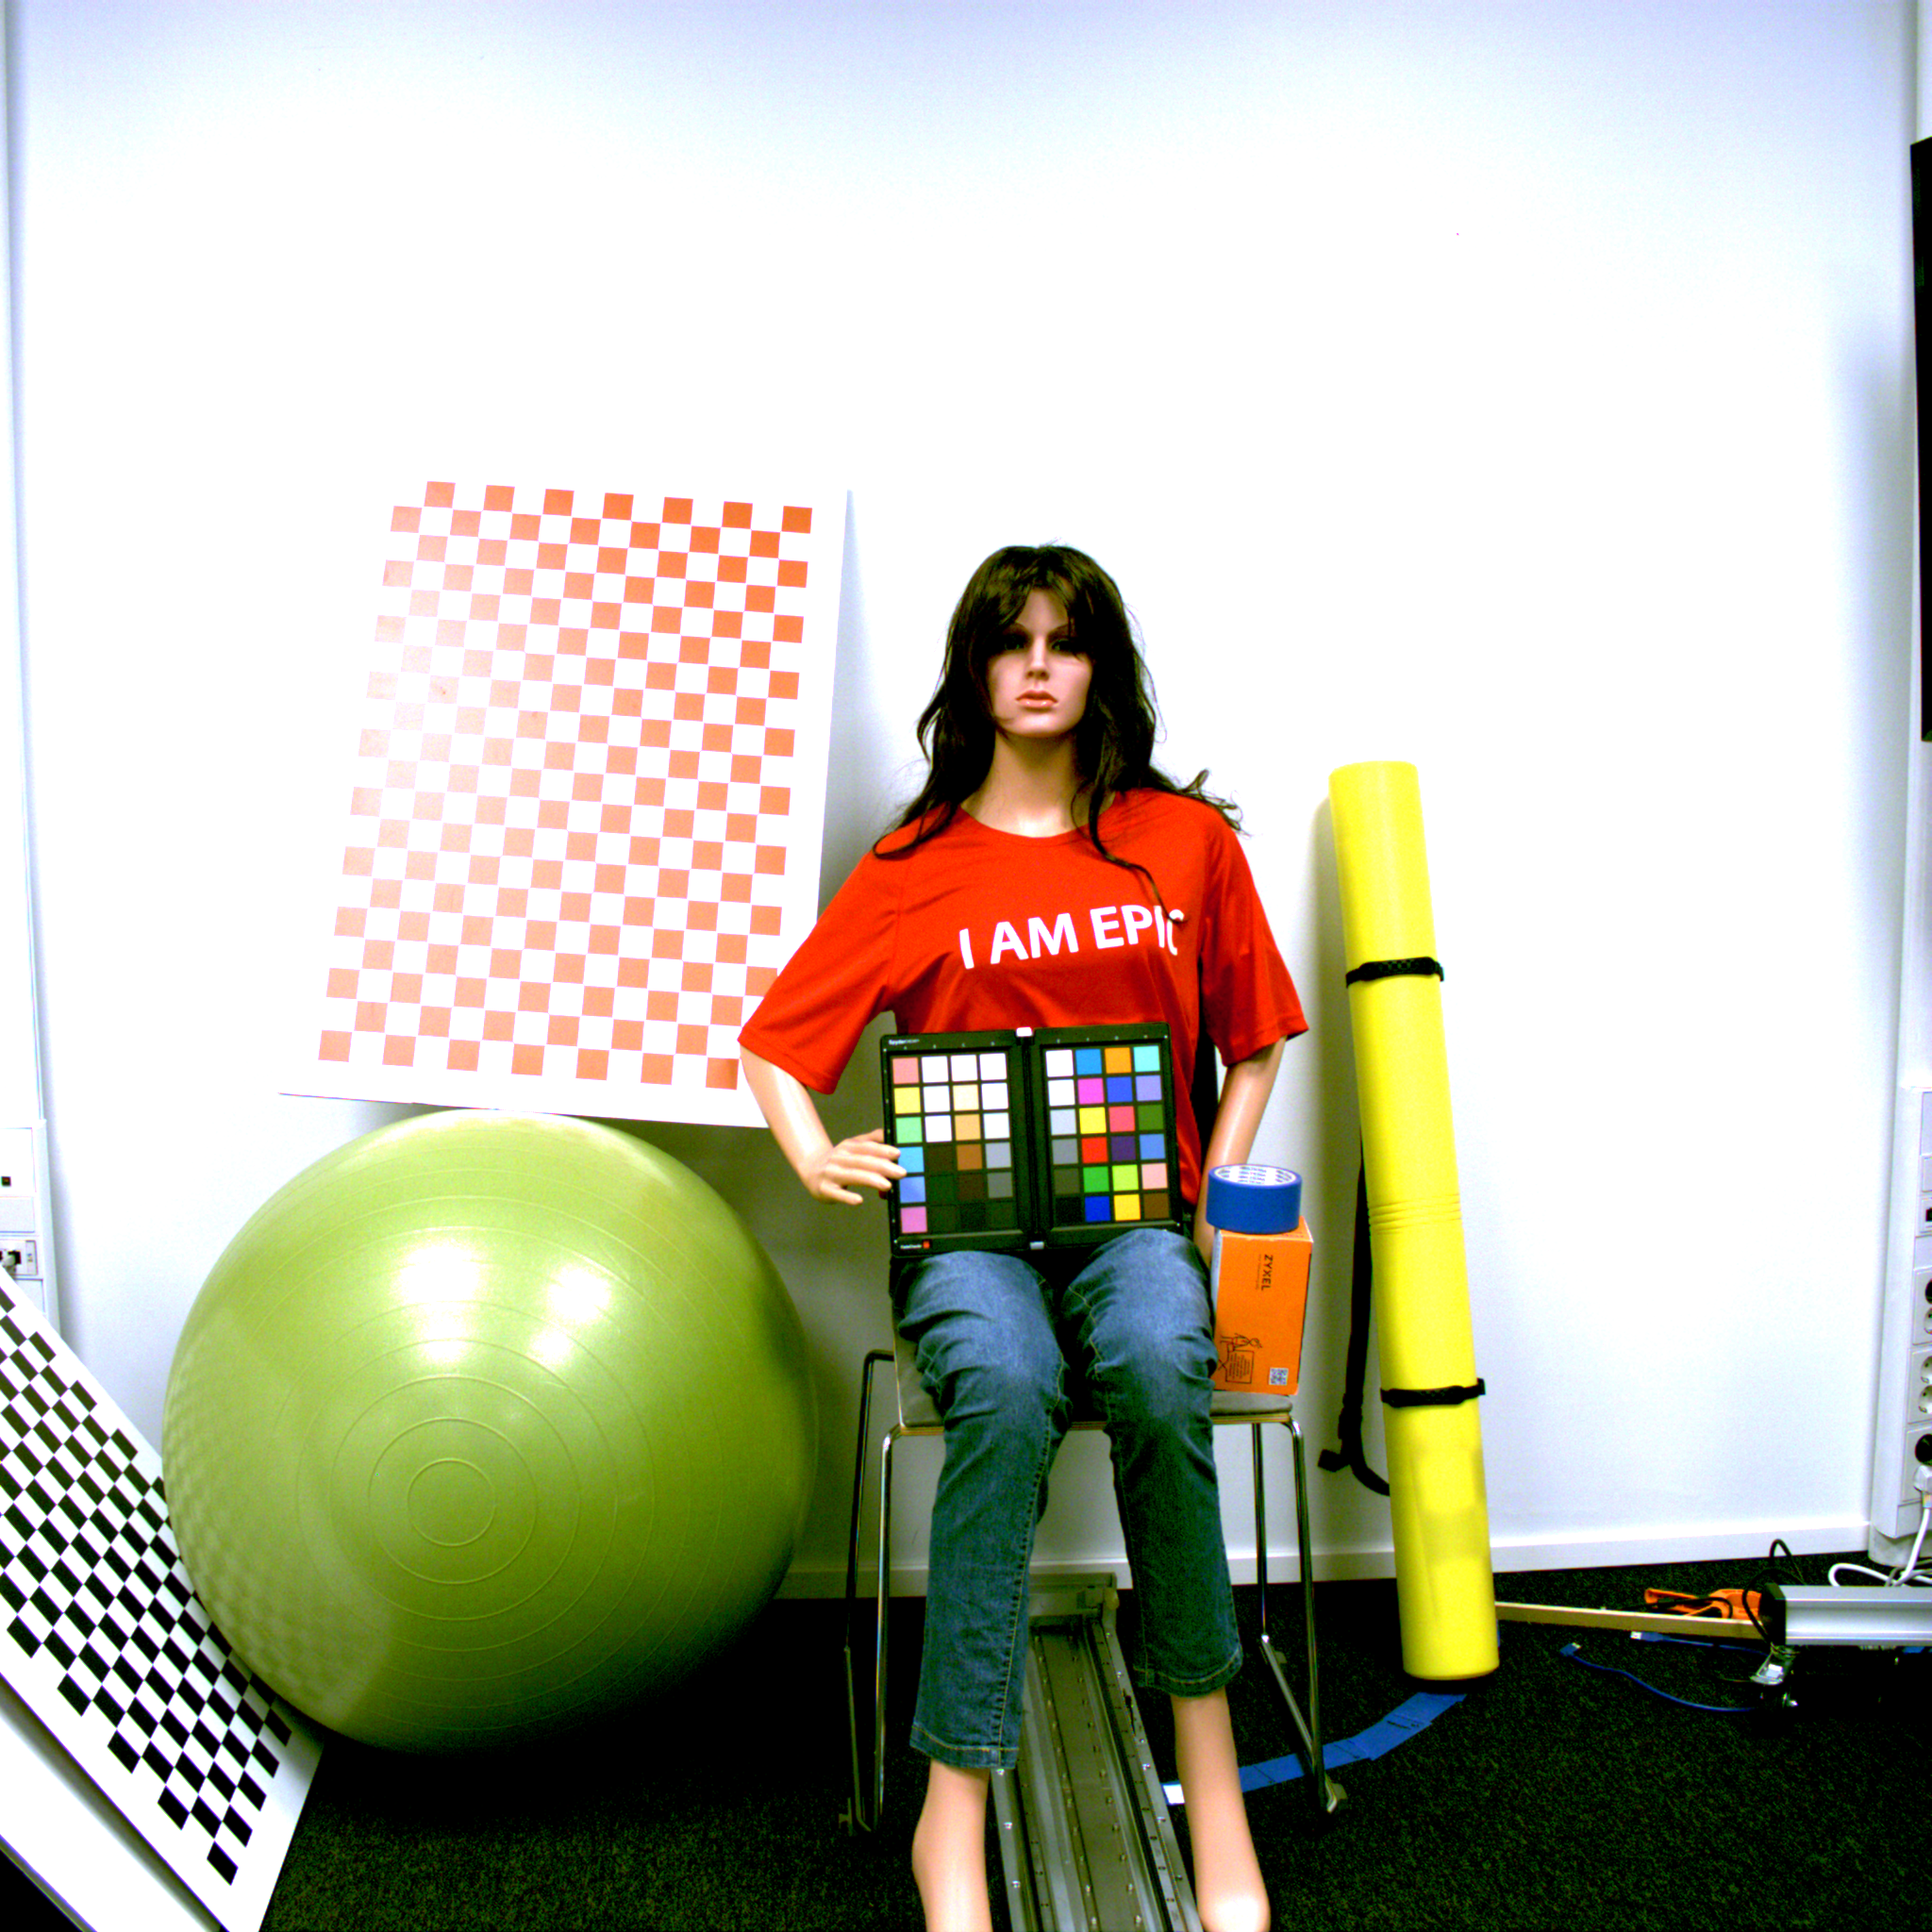
\includegraphics[width=0.4\textwidth, height= 5cm, keepaspectratio]{images/input-image-raw-right.png}
 		 \label{fig:distort-raw-right}
}
	\subfigure[Left rectified stereo image]{
 		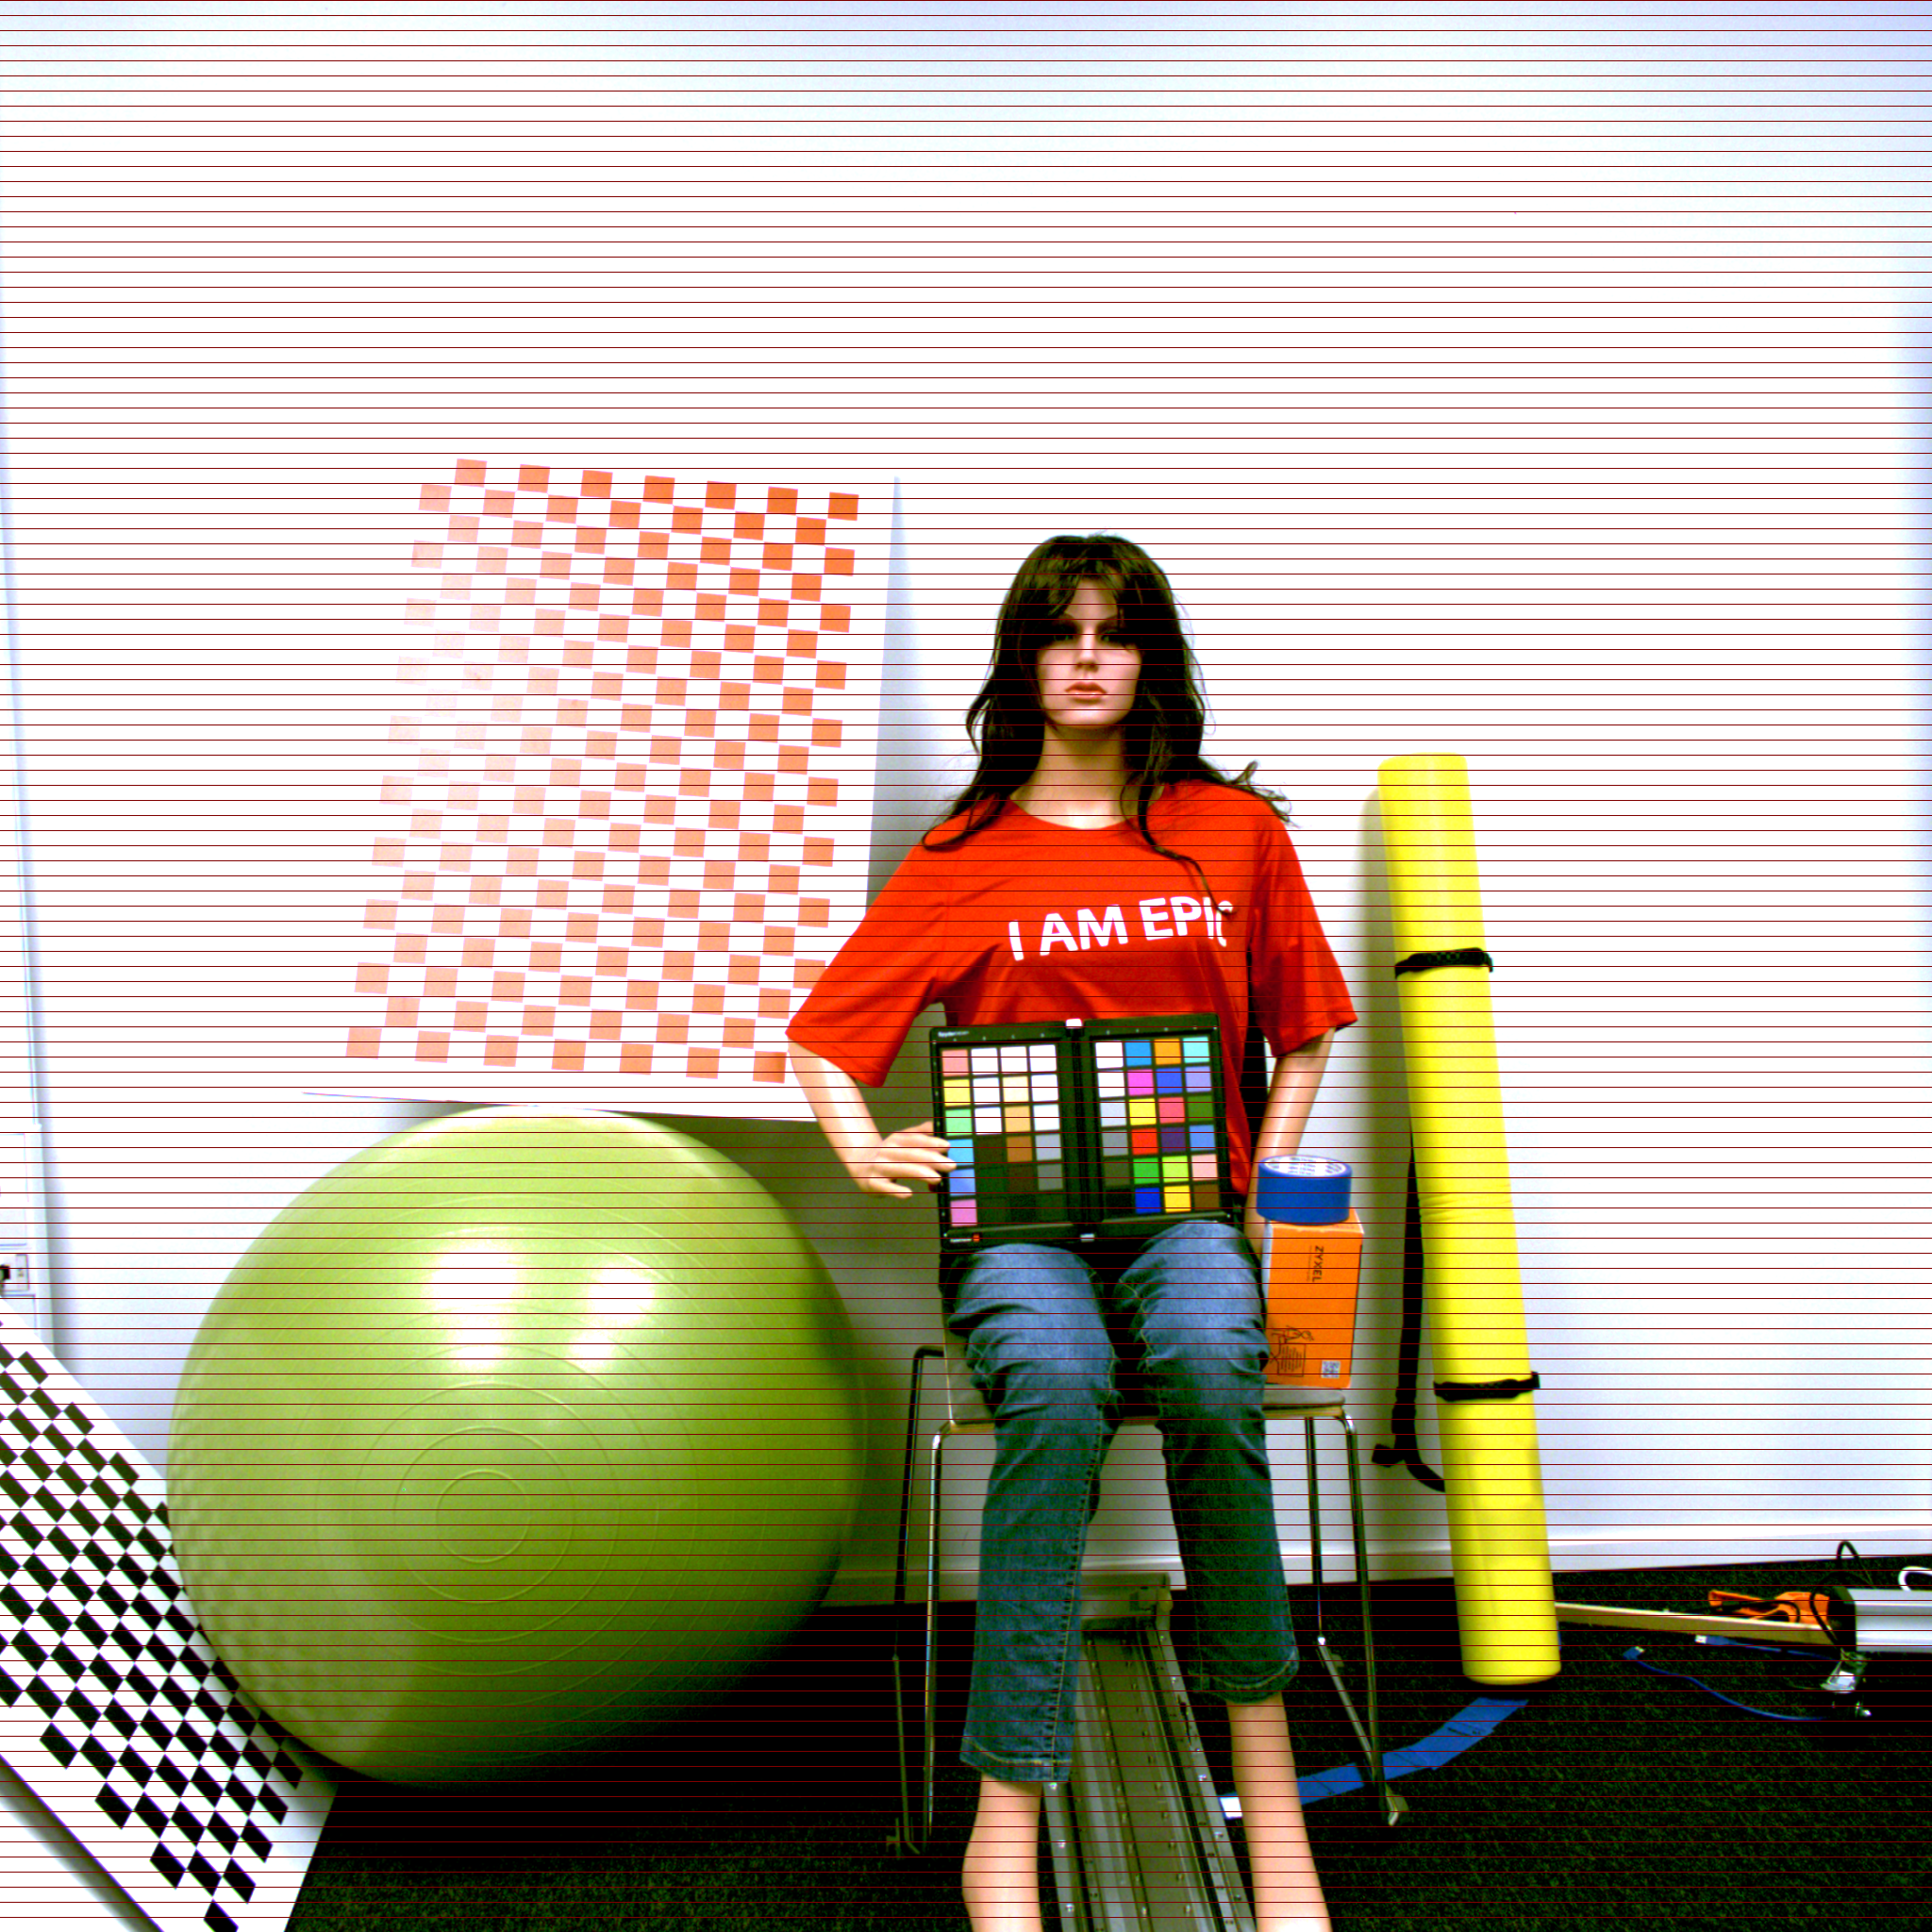
\includegraphics[width=0.4\textwidth, height= 5cm, keepaspectratio]{images/output-image-rect-left.png}
 		\label{fig:stereo-rect-left}
}
	\subfigure[Right rectified stereo image]{
 		 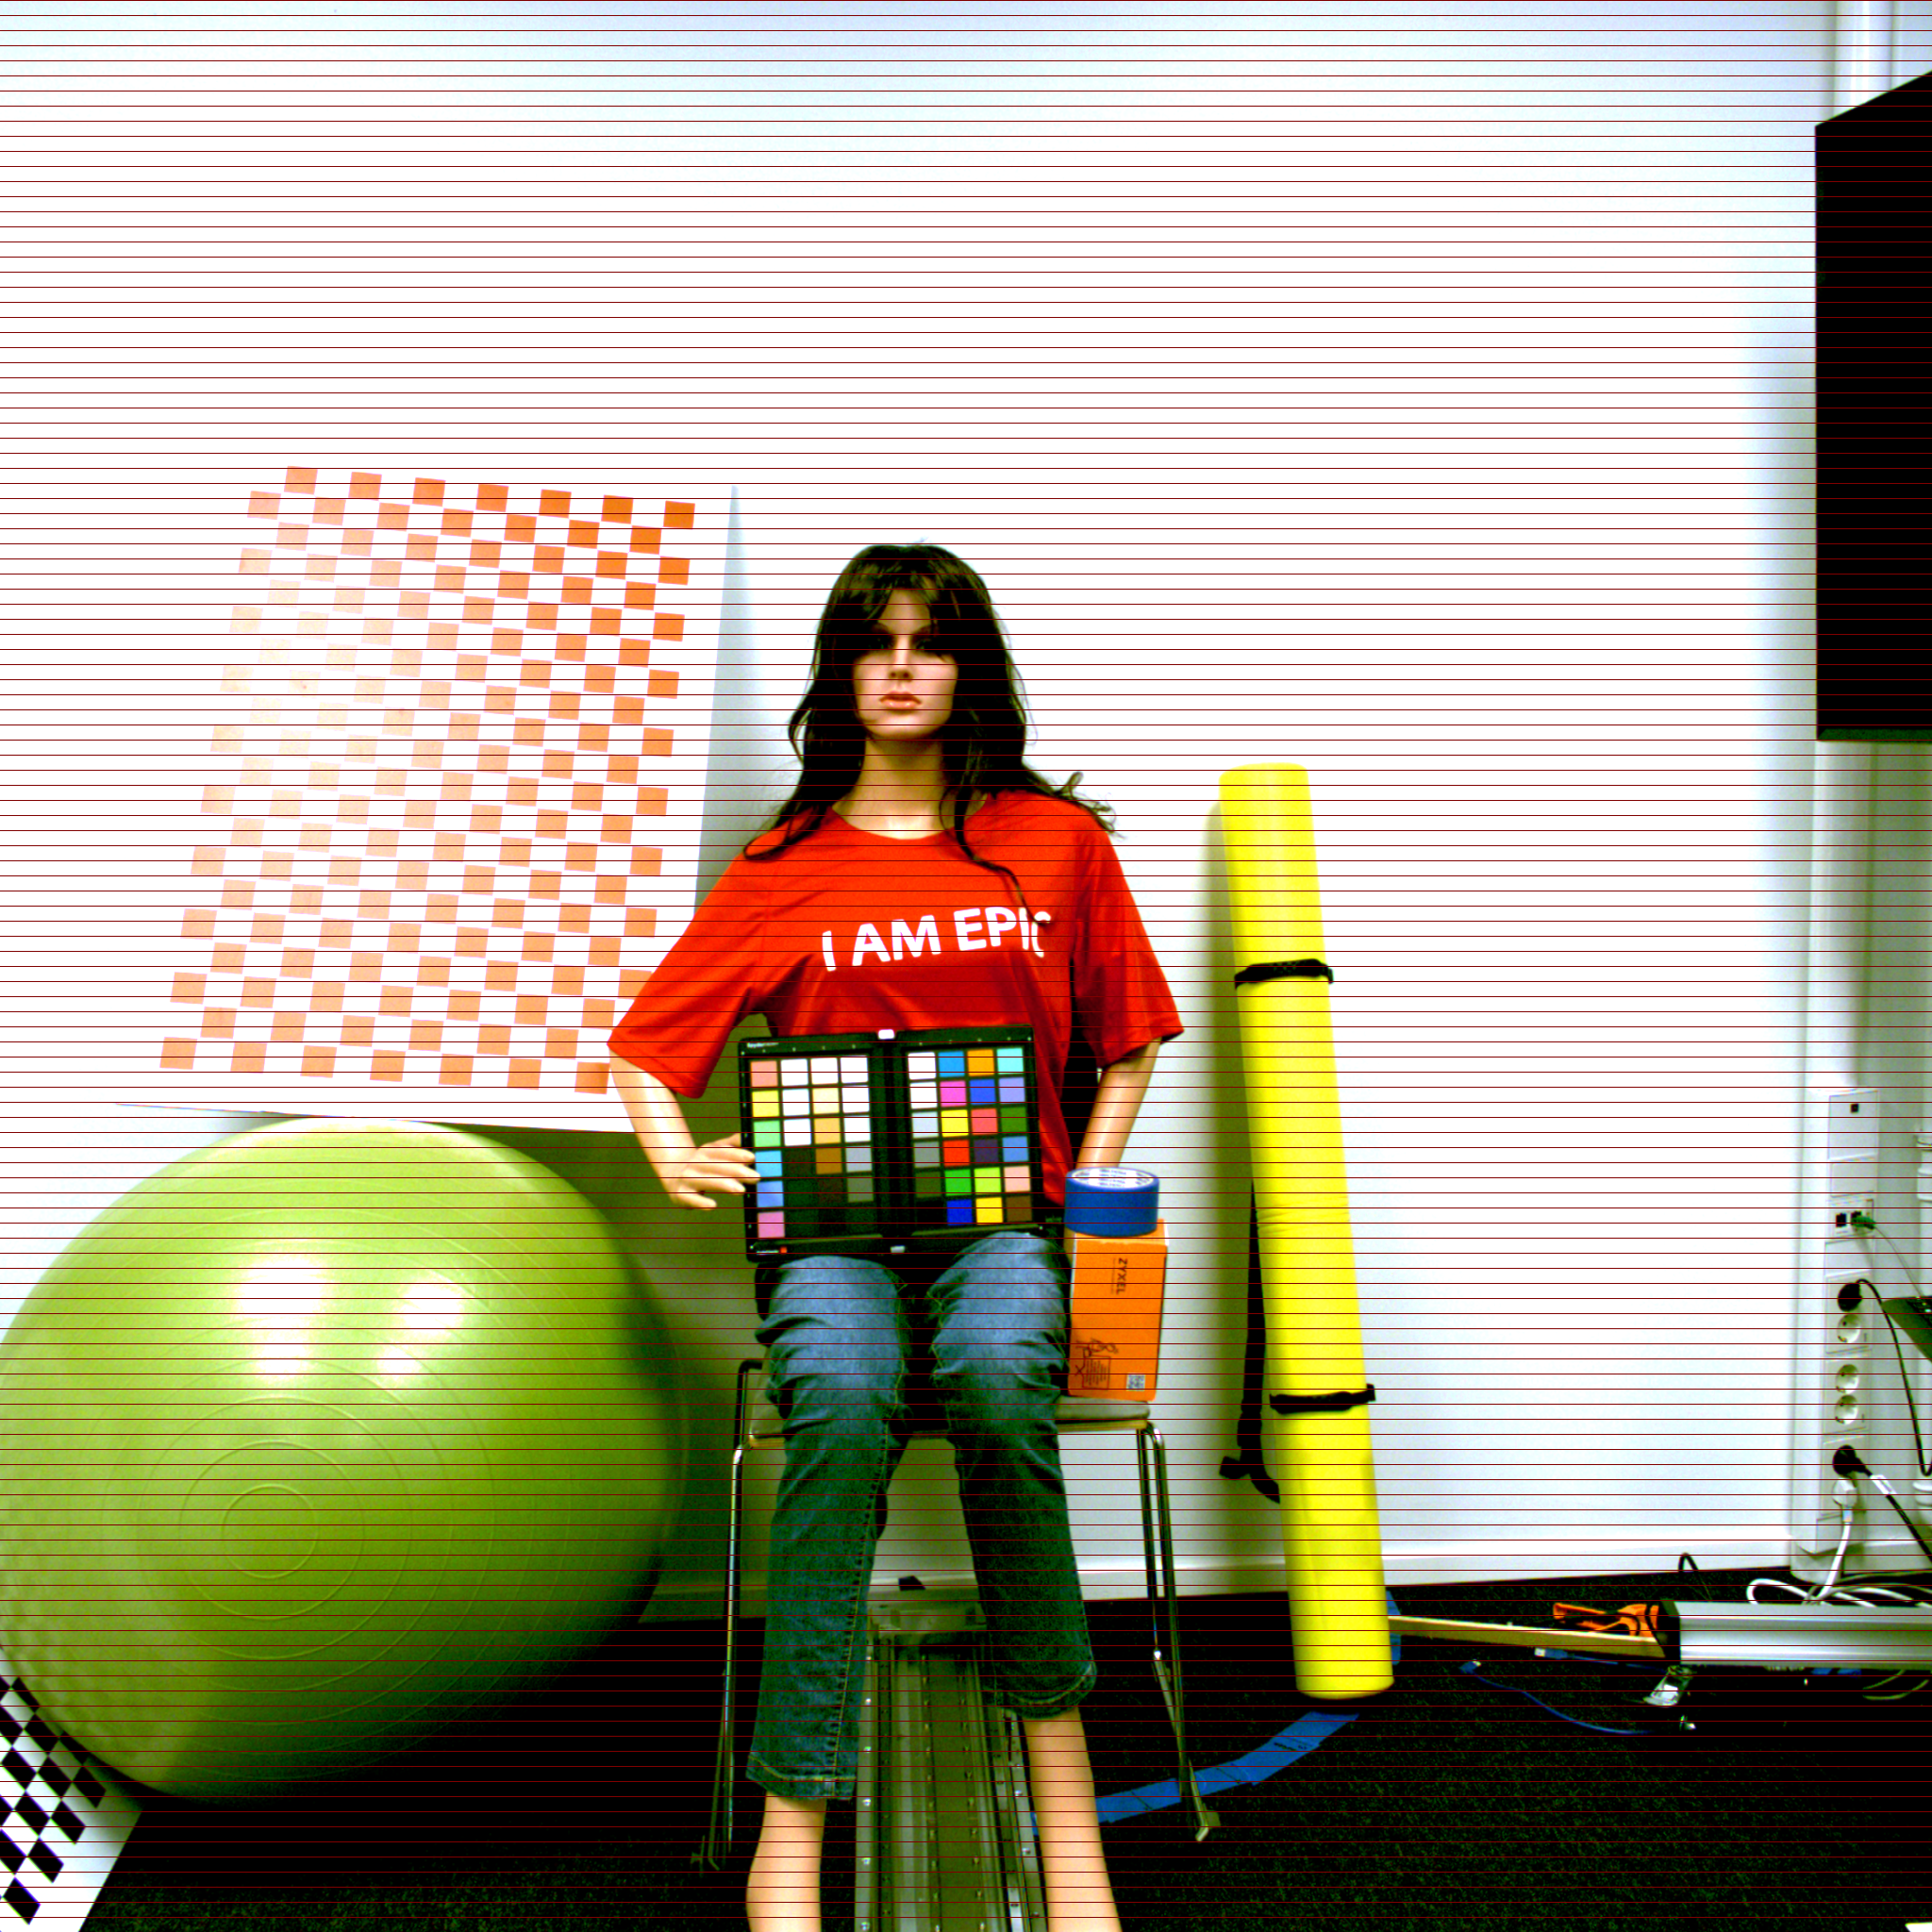
\includegraphics[width=0.4\textwidth, height= 5cm, keepaspectratio]{images/output-image-rect-right.png}
 		 \label{fig:stereo-rect-right}
}
\caption{Distorted raw and stereo rectified images from the Ladimo device}
\label{fig:stereo-undist-rect-4eye}
\end{figure}

Concerning the tests carried out with the real environment images taken from the LaDiMo device, some pre-processing was necessary on the stereo pair too. 
In fact, the hardware employed gives as an output, on top of the point cloud data, a pair of distorted raw RGB images, which has to be first undistorted and then rectified, in order to be correctly used for the stereo matching. \\
Specifically these operations have been completed using the OpenCV built-in functions \texttt{stereoRectify()}, \texttt{initUndistortRectifyMap()} and \texttt{remap()}, which employ the camera calibration data, already available for the used camera, and give as output the matrices that map an image from the distorted reference systems to the stereo rectified space.
In this section a concise explanation of the chain of operations that has been implemented with those functions is proposed.
If further details regarding the specific parameters correlated to those functions are needed, the broad OpenCV documentation available is reminded.\\
Firstly the \texttt{stereoRectify()} function is fed with the original camera matrices and the distortion parameters of the two camera, which are available from the pre-computed calibration procedure.
Moreover, as input to the function there is the transformation matrix from the coordinate system of the principal camera to the secondary camera.
Actually, that is provided as the rotation matrix and the translation vector separately.
Hence, the OpenCV function provides as its main outputs the two rectification transform matrices, that are the matrices that bring the 3D coordinates of a point from the unrectified coordinate system to the rectified coordinate system.
Moreover, the camera projection matrices, which are fundamental in the stereo-matching process, are supplied.\\
After that, the function \texttt{initUndistortRectifyMap()} is exploited for both cameras in order to finalize the rectification procedure.
As a matter of fact, it employs, on top of the initial camera matrices and the distortion coefficients, the rotation and projection matrices for each camera generated from the previous step.
Therefore, with this operation the maps between the initial coordinate system, i.e. distorted, and the destination space, i.e. corrected and rectified, are computed, in order to be, then, fed into the \texttt{remap()} function, which will perform the last step of the rectification process, providing the rectified stereo pair. \\
Figures from \ref{fig:distort-raw-left} to \ref{fig:stereo-rect-right} display the input and the output of the whole rectification procedure.
In the rectified stereo pair in Figures~\ref{fig:stereo-rect-left} and \ref{fig:stereo-rect-right} the image scanlines, which in that coordinate system correspond to the epipolar line, are highlighted in order to provide a visualization of the correctness of the process.
However, if that output is accurately analysed, it is possible to notice some mismatches between the two rectified images.
Those are certainly due to errors in the calibration procedure, which needs to be adjusted for further experiments.

\section{Post-processing testing and analysis}
\label{section:post-processing-impl}

Two main typologies of filters have been applied to the 3D dense point cloud and the disparity image achieved as the output of the estimation algorithm.\\
Specifically, the disparity images obtained during the initial phases of the methods designing have been processed with bilateral or median filter.
The latter result tends to perform better in terms of overall accuracy, even being slightly more expensive from a computational point of view.
The fundamental feature of that filter is the edge preserving, which make it as the preferable choice for a non-invasive noise removal procedure.\\
Differently, the $X$, $Y$ and $Z$ data, estimated for the creation of the dense point cloud, have been handled at the end with a cascade of morphological operations, such as erosion, dilation, opening and closing.
These have been merged together in order to find the best combination, which would be able to simultaneously adjust the result and preserve the achieved output.
Therefore, these operations help in cleaning the whole data from estimations that were clearly wrong and enhance the smoothness and the homogeneity of the final cloud.
	
\section{Preparation to future improvements}
\label{section:intro-future-improv}

Considering the two designed methods for the estimation of a 3D dense point cloud through a stereo photogrammetry procedure, and comparing the results from both perfect dataset images and the ones gathered from the LaDiMo device some general conclusions about the work done and the further improvements that can be implemented in the algorithm can be drawn here, leaving a more interesting and complete discussion to the following chapters.\\
First of all, an important notice that should be done is that, compared with the OpenCV built-in algorithm \texttt{stereoSBGM()}, the lightweight developed algorithm is in general less precise.
However, it is faster and the number of estimations that can be performed inside the specific subregion can be easily adjusted in order to modify its accuracy, obviously loosing performance in computation.\\
Moreover, it has been proved that, if calibration mismatches are present in the stereo images, the OpenCV method tends to generate really noisy disparity images, especially in texture-less regions and near occlusions.
Furthermore, the multiple parameters of that function must be wisely adjusted for every specific image to obtain a reasonable result.\\
On the contrary, the lightweight method developed is able to recover from small errors present in the initial raw images. 
This is due to the fact that this method does not completely rely on the stereo images but it exploits the data from the input cloud of sparse points.
Therefore, thanks to this, small calibration errors do not affect drastically the final result of the algorithm, even if they are not desirable. \\
A final comment has to be introduced regarding the possible improvements that could be added to the algorithm.
For sure, a higher accuracy of the final point cloud would be desired, meaning that smoothness and continuity should be enhanced among the edges, thus to provide a better looking result, making easier the understanding of the object in the specific scene.
Therefore, a first idea that has already been thought to achieve this, keeping potentially real time performance, is to design a hierarchical procedure, where the most accurate points are iteratively used for further estimations, considering that two or three would be sufficient.
Concerning this, if the computational time has to remain low, the estimations in the subsequent runs of the procedure can be focused on the regions close to edges and small objects.
